\documentclass[landscape]{slides}
\usepackage{pgf}
\usepackage{tikz}
\usetikzlibrary{arrows}
\begin{document}

A pretty picture;

\begin{center}
\vspace{-0.4in}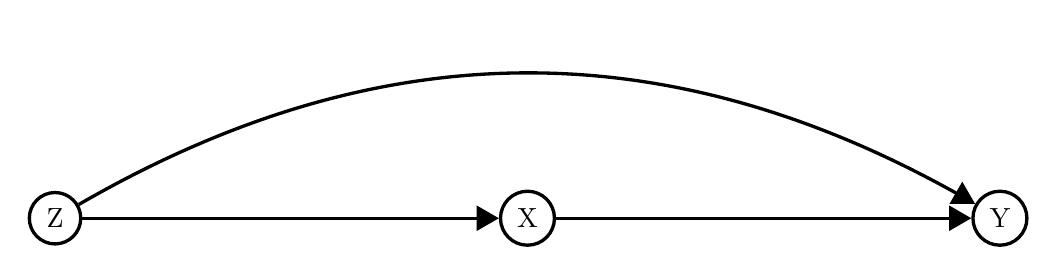
\begin{tikzpicture}[scale=1, >=triangle 60]
\tikzstyle{every node}=[draw,shape=circle];
\tikzstyle{every path}=[very thick];
\path (180:6cm) node (Z) {Z};
\path (0:0cm) node (X) {X};
\path (0:6cm) node (Y) {Y};
\path[->] (Z) edge (X);
\path[->] (X) edge (Y);
\path[->] (Z) edge [out=45, in =135, bend left=30](Y);
\end{tikzpicture} 
\end{center}

and some others;

\definecolor{mygray}{gray}{.80}
\begin{center}
\begin{tikzpicture}[scale=0.9, >=triangle 60]
\tikzstyle{every node}=[draw,shape=circle];
\tikzstyle{every path}=[very thick];
\path (180:4cm) node (X) {X};
\path (0:0cm) node (Z) {Z};
\path (0:4cm) node (Y) {Y};
\path[->] (X) edge (Z);
\path[->] (Z) edge [color=mygray] (Y);
\end{tikzpicture}~
\begin{tikzpicture}[scale=0.9, >=triangle 60]
\tikzstyle{every node}=[draw,shape=circle];
\tikzstyle{every path}=[very thick];
\path (0:0cm) node (Z) {Z};
\path (30:4cm) node (B) {B};
\path (150:4cm) node (A) {A};
\path (210:4cm) node (X) {X};
\path (330:4cm) node (Y) {Y};
\path (0:7cm) node (C) {C};
\path[->] (A) edge (Z);
\path[->] (B) edge (Z);
\path[->] (X) edge (A);
\path[->] (B) edge (C);
\path[->] (Z) edge [color=mygray] (Y);
\path[->] (Z) edge [color=mygray] (C);
\path[->] (X) edge (Z);
\path[->] (X) edge (Y);
\path[->] (C) edge (Y);
\end{tikzpicture} 
\end{center}



\end{document}
